\documentclass[xcolor=pdftex,dvipsnames,table]{beamer}
\mode<presentation>
\usetheme{boxes}
\setbeamertemplate{navigation symbols}{}
% http://www.latex-community.org/forum/viewtopic.php?f=4&t=6694
\setbeamertemplate{navigation symbols}{\raisebox{5pt}{\makebox[\paperwidth]{\hfill\makebox[10pt]{\scriptsize\insertframenumber\vspace{1ex}}}}}
\setbeamertemplate{footline}[frame number]
\setbeamertemplate{blocks}[shadow=false]
\setbeamercolor*{block title}{fg=structure,bg=RoyalBlue!10}
\setbeamercolor*{block title example}{fg=BrickRed,bg=Goldenrod!10}
\setbeamercolor*{block title alerted}{fg=white,bg=black}
\addtobeamertemplate{block begin}{\pgfsetfillopacity{0.8}}{\pgfsetfillopacity{1}}
\rowcolors{1}{RoyalBlue!20}{RoyalBlue!5}

%\DeclareGraphicsRule{*}{mps}{*}{}

\usepackage{latexsym}
\usepackage{hyperref}

\raggedright

\newcount\lecturecount
\lecturecount=0
\AtBeginLecture{%
    \advance\lecturecount by 1
    \date{}
    \begin{frame}
    \begin{center}
    \titlepage
    \ifnum\lecturecount=1
    Part \the\lecturecount: \insertlecture
    \else
    Part \the\lecturecount: \insertlecture
    \fi
    \end{center}
    \end{frame}
}

\begin{document}

\title{\color{blue}Natural Language Processing}

\author{Anoop Sarkar \\ {\tt http://anoopsarkar.github.io/nlp-class}}
\institute{}
%\date{}
     
{
\setbeamertemplate{navigation symbols}{}
\addtocounter{framenumber}{-1}
\begin{frame}
\begin{center}
\vspace{1cm}
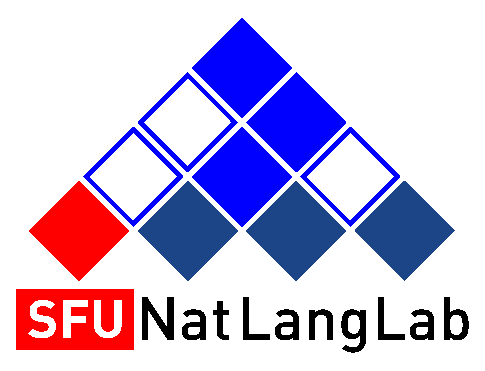
\includegraphics[scale=0.4]{figures/natlang-cky-logo.eps}
\end{center}
\titlepage
\end{frame}
}



\lecture{Neural Language Models}{}
\section{Log-linear Language Models}

\begin{frame}
\frametitle{The Language Modeling problem}
\begin{block}{Setup}
\begin{itemize}[<+->]
\item Assume a (finite) vocabulary of words:
\[ {\cal V} = \{ killer, crazy, clown \} \]
\item Use ${\cal V}$ to construct an infinite set of \textit{sentences} 
\begin{eqnarray*} 
{\cal V}^+ = & \{ & \\
&& \mbox{clown, killer clown, crazy clown, } \\
&& \mbox{crazy killer clown, killer crazy clown}, \\
&& \ldots \\
& \} &
\end{eqnarray*}
\item A \textit{sentence} is \textbf{defined} as each $s \in {\cal V}^+$
\end{itemize}
\end{block}
\end{frame}


\section*{Acknowledgements}

\begin{frame}
\centering
\begin{alertblock}{Acknowledgements}
Many slides borrowed or inspired from lecture notes by Michael Collins, Chris Dyer, Kevin Knight, Philipp Koehn, Adam Lopez, and Luke Zettlemoyer from their NLP course materials. 

\bigskip

All mistakes are my own.
\end{alertblock}
\end{frame}



\end{document}
